\section{Background: Distributed Databases \& Big Data}\label{sec:distributed}

\subsection{Introduction}
We ask: does the world have any precedents for \textit{distributed databases} at massive scale? The answer is yes.
All large Internet companies, and many small ones, run “big data” distributed databases (DBs), including Facebook, Google, Amazon and Netflix.
For example, at any given time Netflix might be serving up content making up $35\%$ of the bandwidth of the entire Internet \cite{spangler2014netflix}.

Distributed DBs regularly store petabytes ($1,000,000$ GB) or more worth of content. 
In contrast, the Bitcoin blockchain currently stores $50$ GB, the capacity of a modern thumb drive.
There are initiatives to prevent “blockchain bloat” caused by “dust” or “junk” transactions that “pollute” Bitcoin’s $50$ GB database \cite{wagner2014blockchain_bloat}.

In light of petabyte-capacity DBs, it is ironic that a $50$ GB database would be concerned by “bloat”.
But let’s look at it another way: perhaps distributed DB technology has lessons for blockchain DB design.

\medskip
\centerline{Let’s explore distributed DB scalability further.}

\begin{figure}[!ht]
  \centering
  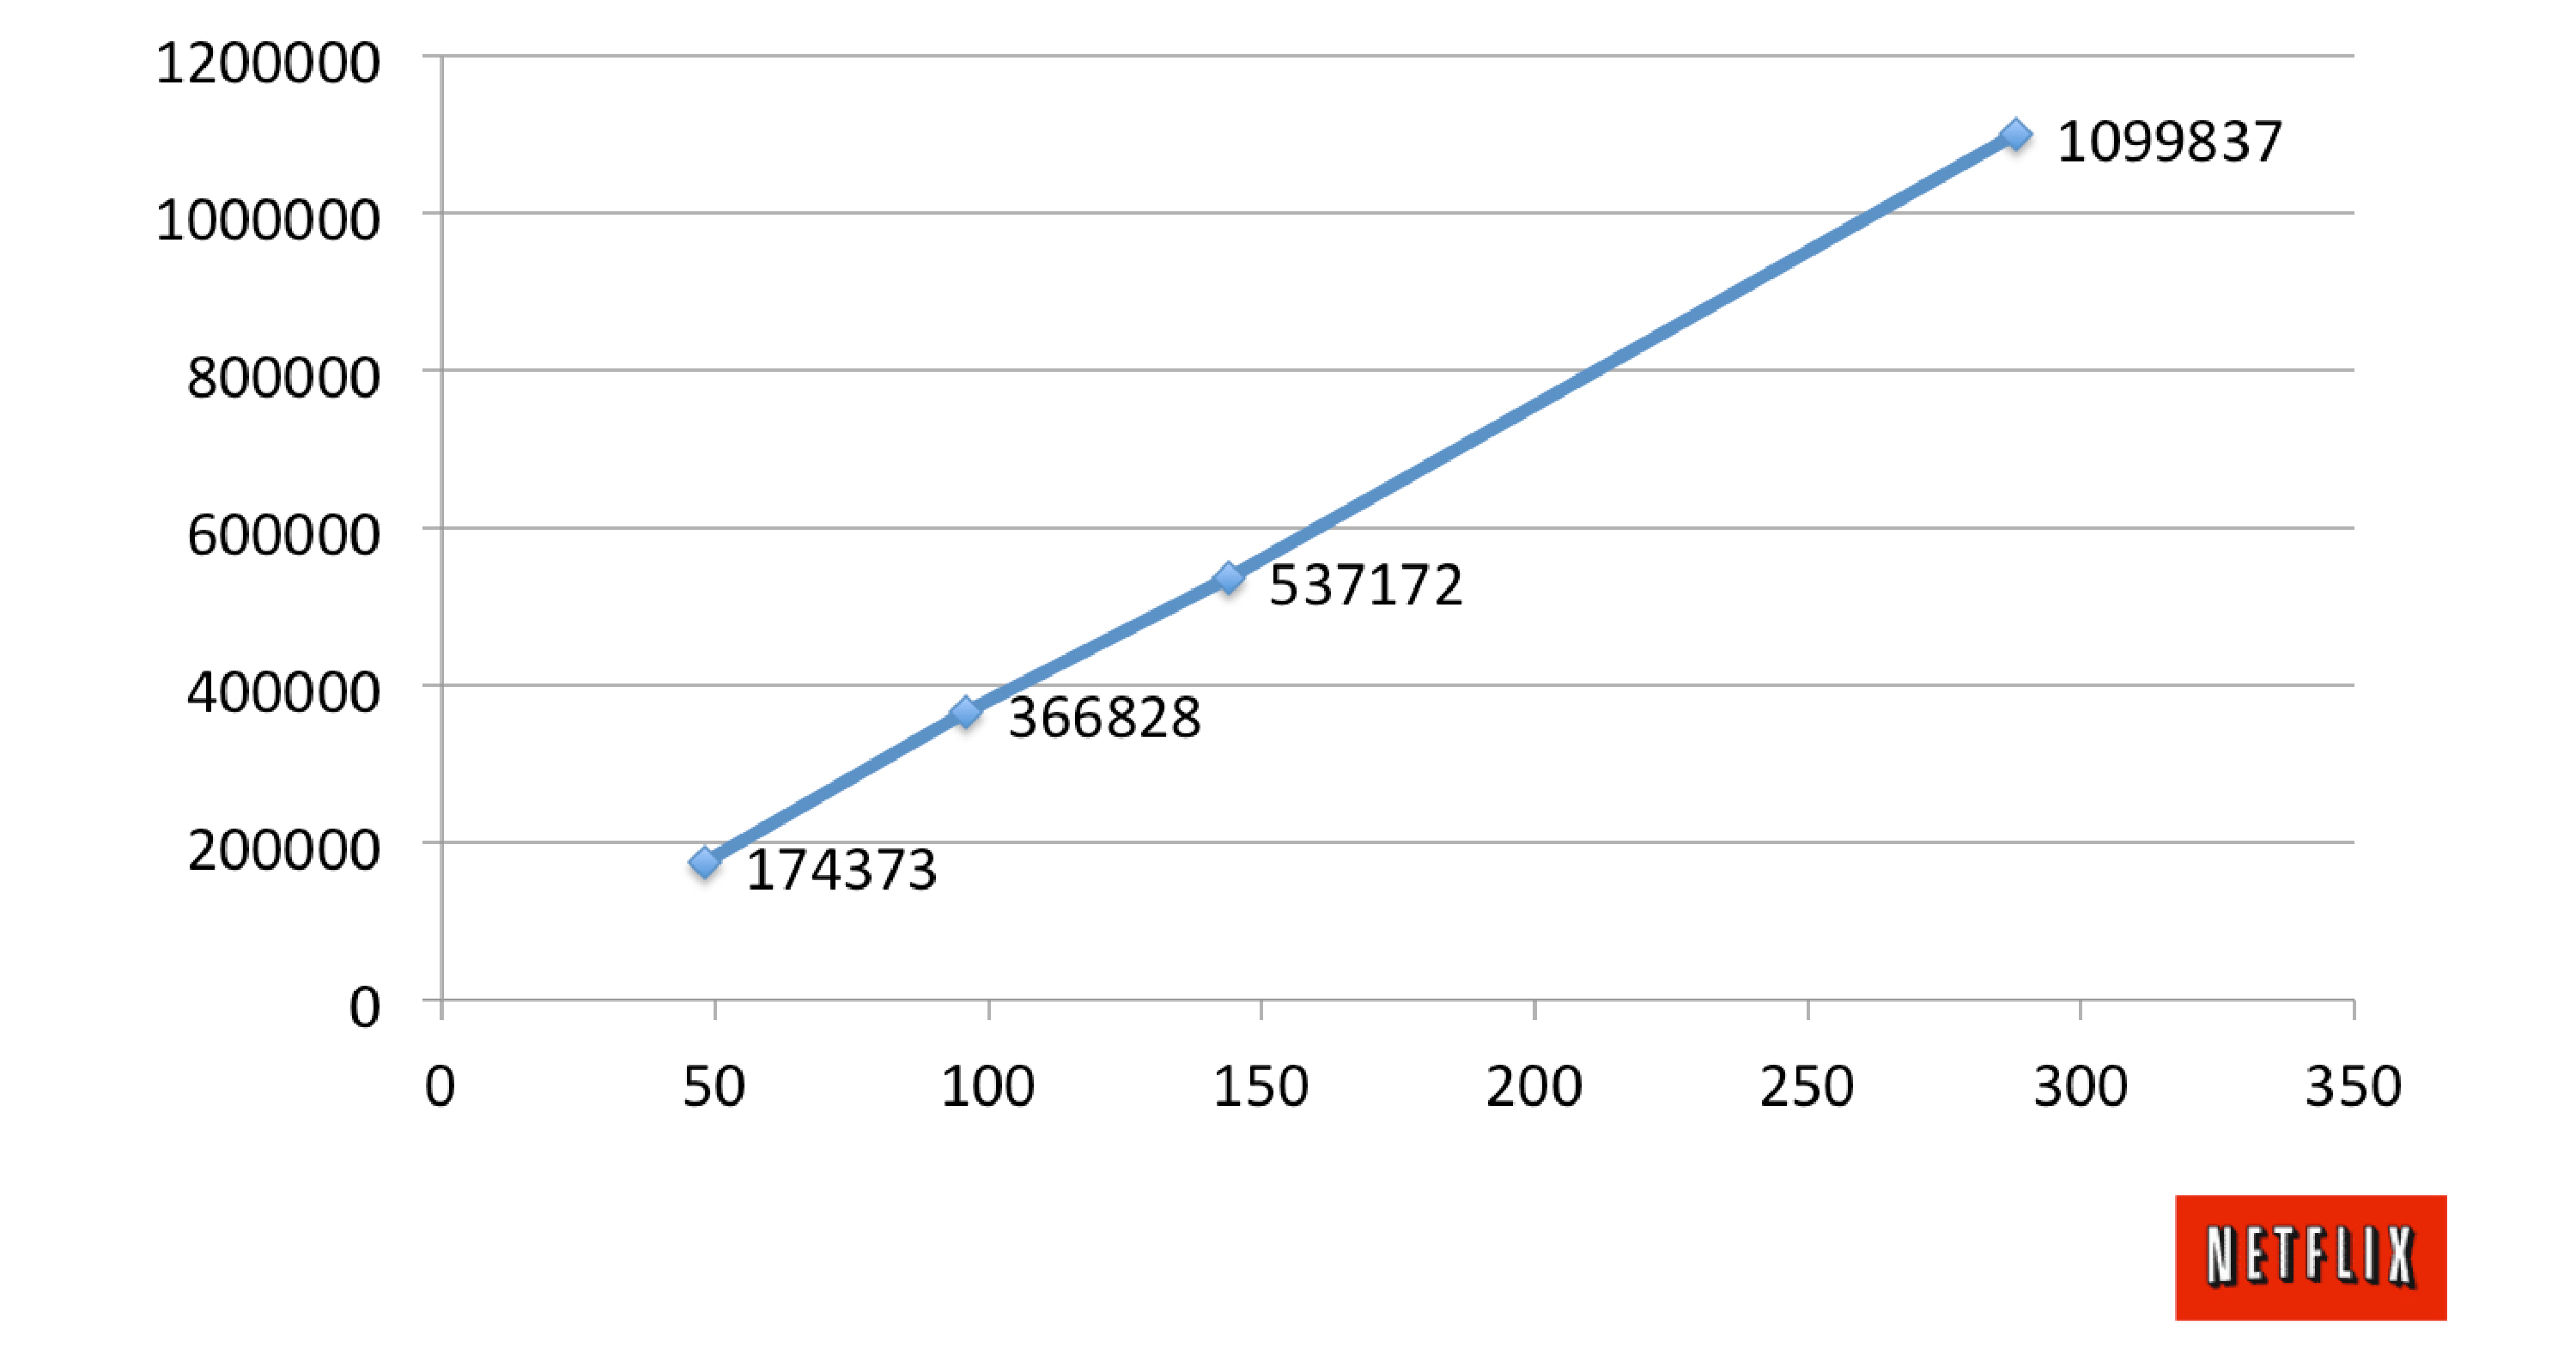
\includegraphics[width=\textwidth]{figure_2.pdf}
  \caption{Netflix experimental data on throughput of its Cassandra database (Client writes/s by node count - Replication Factor=$3$).
  The x-axis is number of nodes; the y-axis is transactions per second. From \cite{cockcroft2011benchmarking}.}
  \label{fig:cassandra_throughput}
\end{figure}

\medskip
Figure \ref{fig:cassandra_throughput} illustrates the throughput properties of Cassandra, a distributed DB technology used by Netflix.
At the bottom left of the plot, we see that $50$ distributed Cassandra nodes handle $174,000$ tps.
Increasing to $300$ nodes gives $1.1$ million transactions per second (tps) \cite{cockcroft2011benchmarking}.
A follow-up study three years later showed a throughput of $1$ million tps with just a few dozen nodes \cite{kalantzis_netflix}.
To emphasize: the throughput of this DB increased as the number of nodes increased. The scaling is linear: $10\times$ more nodes means $(10c)\times$ more throughput, where $0 < c \leq 1$.

Each node also stores data.
Critically, a node only stores a subset of all data, that is, it has partial replication.
In the Netflix example \cite{kalantzis_netflix}, each piece of data has three copies in the system, i.e. a replication factor of three.
Partial replication enables an increase in the number of nodes to increase storage capacity.
Most modern distributed DBs have a linear increase in capacity with the number of nodes, an excellent property.
Additionally, as the number of nodes increases, Cassandra’s latency and network usage does not worsen.
Cassandra can be distributed at scale not only throughout a region, but around the globe.
Contrast this to the Bitcoin blockchain, where capacity does not change as the number of nodes increases.

The scalability properties of distributed DBs like Cassandra make an excellent reference target.

\subsection{Consensus Algorithms in Distributed Databases}
\subsubsection{Introduction}
Cassandra achieves its scale because it avoids scalability-killing decisions like making a full copy of all the data at every node, the baggage of mining, coins, and the like.

What Cassandra does have is a consensus algorithm that uses $2f+1$ processes to tolerate $f$ benign processes \cite{lamport1998part}, which is used to get the distributed data to synchronize.

Synchronizing distributed data was in fact the original motivation for the BG problem.
The problem was first documented in $1980$ by Leslie Lamport and colleagues \cite{pease1980reaching}, and solved two years later, also by Lamport and colleagues.
The solution is the Paxos protocol \cite{lamport1982byzantine} with versions that can tolerate $f$ Byzantine faults using $3f+1$ processes \cite{lamport2011byzantizing, castro2001byzantine}\footnote{Benign faults are system crashes, lost messages, and the like. In systems with benign faults, all nodes are assumed to follow the same protocol.
Byzantine faults include benign faults, but also deviations from the protocol, including lying, collusion, selective non-participation, and other arbitrary behavior.}.

\subsubsection{Paxos Consensus Algorithm}\label{subsec:distributed:paxos}
This section describes the origins of Paxos.
In $1980$, Lamport challenged colleagues with the following question: \quote{Can you implement a distributed database that can tolerate the failure of any number of its processes (possibly all of them) without losing consistency, and that will resume normal behavior when more than half the processes are again working properly?} \cite{lamport_writings}

It was generally assumed at the time that a three-processor system could tolerate one faulty processor.
Lamport’s paper introduced the problem of handling “Byzantine” faults, in which a faulty processor sends inconsistent information to the other processors, which can defeat any traditional three-processor algorithm.
In general, $3f+1$ processors are needed to tolerate $f$ faults.
However, if digital signatures are used, $2f+1$ processors are enough.
This was the first precise statement of the consensus problem \cite{lamport1982byzantine}.

Lamport then set out to prove the problem was impossible to solve \cite{lamport_writings}.
Instead, in a happy accident, he discovered the Paxos algorithm \cite{lamport1998part}.

At the heart of Paxos is a three-phase consensus protocol.
Lamport wrote, “to my knowledge, Paxos contains the first three-phase commit algorithm that is a real algorithm, with a clearly stated correctness condition and a proof of correctness” \cite{lamport_writings}.
Paxos overcame the impossibility result of Fischer et al. \cite{fischer1985impossibility} by using clocks to ensure liveness.

\subsection{Extensions to Paxos Consensus}
The original Paxos could handle arbitrary benign (non-Byzantine) failures such as network delays, packet loss, system crashes and so on.

Several Byzantine fault tolerant systems were designed in the 1980s \cite{wiki_byzantine}, including Draper's FTMP \cite{paulitsch2005coverage}, Honeywell's MMFCS \cite{hopkins1987evolution}, and SRI's SIFT \cite{driscoll1983multi}.

However, those early systems were slow when it came to faults.
Lamport’s “Fast Paxos” \cite{lamport2006fast} and Castro’s “Practical Byzantine Fault Tolerance” (PBFT) \cite{castro2001byzantine} improved upon speed under malicious conditions.
Aardvark \cite{clement2009making} and RBFT \cite{aublin2013rbft} are examples of continued research in speed and reliability.

Paxos is notoriously difficult to understand, and risky to implement.
To address this, Raft \cite{ongaro2014raft} was designed specifically for ease of understanding, and consequent lower implementation risk.
It has a robust variant \cite{copeland2014tangaroa}.

The recent Stellar protocol allows each node to choose which other nodes to trust for validation \cite{mazieres2015stellar}.

\subsection{Usage / Ecosystem}
Mike Burrows of Google (co-inventor of Google’s Chubby, BigTable, and Dapper) has said ``There is only one consensus protocol, and that’s Paxos,'' \cite{robinson2009paxos} and ``all working protocols for asynchronous consensus we have so far encountered have Paxos at their core'' \cite{burrows2006chubby}.
Henry Robinson of Cloudera has said ``all other approaches are just broken versions of Paxo'' and ``it’s clear that a good consensus protocol is surprisingly hard to find.'' \cite{robinson2009paxos}\footnote{An especially interesting statement in light of efforts the Bitcoin community is spending on consensus algorithms.}.

Paxos and its lineage is used at Google, IBM, Microsoft, OpenReplica, VMWare, XtreemFS, Heroku, Ceph, Clustrix, Neo4j, and certainly many more \cite{wiki_paxos}.

\subsection{Replication factor \& blockchain “full nodes”}
A modern distributed DB is designed to appear like a single monolithic DB, but under the hood it distributes storage across a network holding many cheap storage devices.
Each data record is stored redundantly on multiple drives, so if a drive fails the data can still be easily recovered.
If only one disk fails at a time, there only needs to be one backup drive for that data.
The risk can be made arbitrarily small, based on assumptions of how many disks might fail at once.
Modern distributed DBs typically have 3 backups per data object, a replication factor of $3$ \cite{wiki_raid}.

In contrast, Bitcoin has about $6,500$ full nodes \cite{bitcoin2015fees}—a replication factor of $6,500$.
The chance of all nodes going down at once in any given hour (assuming complete independence) is $(1/8760)^{6500}$, or $10^{-25626}$.
The chance of all nodes going down would occur once every $3,000$ billion years. To say this is overkill is to put it mildly.

Of course, hardware failure is not the only reason for lost data.
Attacks against the nodes of the network have a much higher probability of destroying data.
A well-targeted attack to $2$ or $3$ mining pools could just remove $50\%$ of the computing power from the current Bitcoin network, making the network unusable until the next adjustment to POW complexity, which happens about every two weeks.

\subsection{Strengths and Weaknesses}
Let’s review the strengths and weaknesses of DBs that use Paxos-style distributed consensus algorithms.

\medskip
\noindent\textbf{Strengths.} As discussed above, Paxos is a proven consensus algorithm that tolerates benign faults and extensions for Byzantine tolerance have been reported.
It is used by “big data” distributed DBs with the well-documented ability to handle high throughput, low latency, high capacity, efficient network utilization, and any shape of data, including table-like SQL interfaces, object structures of NoSQL DBs, and graph DBs, and they handle replication in a sane fashion.
Derivatives like Raft make distributed consensus systems easier to design and deploy.

\medskip
\noindent\textbf{Weaknesses.} While their technical attributes and performance are impressive, traditional “big data” distributed DBs are not perfect: they are centralized.
They are deployed by a single authority with central control, rather than decentralized control as in blockchains.
This creates a number of failings.
Centralized DBs are:
\begin{itemize}
  \item \textbf{Susceptible to a single point of failure}, where a single node being hacked can be disastrous. This flaw is what lead to hacks at Target, Sony, the U.S. Office of Personnel Management (OPM),and many others \cite{bluestone2014sony_hack, davis2015hacking}.
  \item \textbf{Mutable.} A hacker could change a 5-year-old record without anyone noticing (assuming no additional safeguards in place). For example, this would have prevented police from doctoring evidence in the India exam scandal \cite{sethy2015india_scam}. Such tampering is not possible in blockchains because past transactions cannot be changed or deleted, as each new block contains a “hash” digest of all previous blocks.
  \item \textbf{Not usable by participants with divergent interests} in situations where they do not want to cede control to a single administrator. For example, the risk of losing control of the management of information is one reason that copyright rightsholders in the music industry do not share a single DB.
  \item \textbf{Not designed to stop Sybil attacks}, where one errant node can swamp all the votes in the system.
  \item \textbf{Traditionally without support for the creation and transfer of digital assets} where only the owner of the digital asset, not the administrator of the DB, can transfer the asset.
  \item \textbf{Not typically open to the public} to even read, let alone write. Public openness is important for public utilities. A notable exception is WikiData \cite{wikidata}.
\end{itemize}

\subsection{Fault Tolerance in the BigchainDB System}

Simultaneously preserving the scalability and trustless decentralization of both large-scale databases and decentralized blockchains is the main objective of the BigchainDB system. The following were considered when designing BigchainDB's security measures:

\begin{itemize}
  \item \textbf{Benign faults}: In the BigchainDB setup, nodes communicate through a database which uses a fault-tolerant consensus protocol such as Raft or Paxos. Hence we can assume that if there are $2f + 1$ nodes, $f$ benign-faulty nodes can be tolerated (at any point in time) and each node sees the same order of writes to the database.
  \item \textbf{Byzantine faults}: In order to operate in a trustless network, BigchainDB incorporates measures against malicious or unpredictable behavior of nodes in the system. These include mechanisms for voting upon transaction and block validation. Efforts to achieve full Byzantine tolerance are on the roadmap and will be tested with regular security audits.
  \item \textbf{Sybil Attack}: Deploying BigchainDB in a federation with a high barrier of entry based on trust and reputation discourages the participants from performing an attack of the clones. The DNS system, for example, is living proof of an Internet-scale distributed federation. Appendix \ref{sec:dns} describes how the DNS has successfully run a decentralized Internet-scale database for decades.
\end{itemize}